\chapter{楕円曲線}
%楕円曲線の定義, 加算, 楕円曲線上の離散対数問題, Singular, Ordinary, Supersingularな曲線, フロベニウス写像について書く.点の加算を二進展開ですることを書く.  
\section{楕円曲線の定義}
\par
楕円曲線とは,一般的に
\[
E:y^2+a_1xy+a_3y=x^3+a_2x^2+a_4x+a_6 \ \ \ (a_1,a_2,a_3,a_4,a_6\in \mathbb {F}_q)
\]
で与えられる$(x,y)$に関する方程式のことである.係数$a_n$が属する体$\mathbb {F}_q$を係数体,変数$x,y$が属する体を定義体と呼ぶ.このとき、体$K$上の楕円曲線とは,この方程式に無限遠点と呼ばれる要素$\mathcal{O}$を加えた$x,y\in K$である点$(x,y)$の集合を表す.\\
もし、$K$の標数が2であるとき,方程式は
\[
y^2+xy=x^3+ax^2+b \ \ \ (a,b\in \mathbb {F}_q)
\]
と変形され,上式を満たす点の集合となる.\\
また、$K$の標数が3であるときは,方程式は
\[
y^2=x^3+ax^2+bx+c \ \ \ (a,b,c\in \mathbb {F}_q)
\]
と変形され,標数が3より大きい場合は$y^2=x^3+bx+c$と変形される.\\
\par
\section{楕円曲線上の点の加算}
\par
楕円曲線上の有理点において,通常の座標で行われる点の加算とは異なる加算の定義をする.楕円曲線上の点$P,Q$を取ってきたとき,まず点$P,Q$を通る直線を引き, 第三の交点$P\ast Q$を見つける.次に,$P\ast Q$と無限遠点$O$を通る直線($x$軸との垂線)を引き, 楕円曲線と交わるもう1つの交点を楕円曲線における点$P$と$Q$が加算された点$P+Q$とする. \\
一方, $P=Q$である場合は楕円曲線との点$P$における接線を引き,その交点を$P\ast Q$とする.\\
また,この加算により楕円曲線は群構造をなす.例えば,点$P=(x,y)$と$Q=(x,-y)$の場合,第三の交点は無限遠点となる.よって,$P+Q=\mathcal{O}$となり点$Q$が点$P$の逆元,$−P$となる.すなわち単位元が無限遠点,逆元は$x$軸と対称な点になる.結合法則は,加算の定義により自明である.また,無限遠点同士の加算は無限遠点となる.\\
この定義を実数上で描かれた楕円曲線のグラフを用いて示す.ただし,$P,Q\in E(\mathbb{F}_q)$について$P=(x_1,y_1),Q=(x_2,y_2)$とする.

\begin{description}
\item[Case 1.] $P\not=Q,\quad x_1\not=x_2 \longrightarrow$図\ref{fig:elliptic01.eps}
\item[Case 2.] $P=Q\longrightarrow $図\ref{fig:elliptic02.eps}
\item[Case 3.] $P\not=Q,\quad x_1=x_2\longrightarrow $図\ref{fig:elliptic03.eps}
\item[Case 4.] $P=\mathcal{O}$あるいは$Q=\mathcal{O}\longrightarrow $図\ref{fig:elliptic04.eps}
\item[Case 5.] $P=Q=\mathcal{O}$
\end{description}


\begin{figure}[htbp]
  \begin{minipage}{0.5\hsize}
    \begin{center}
      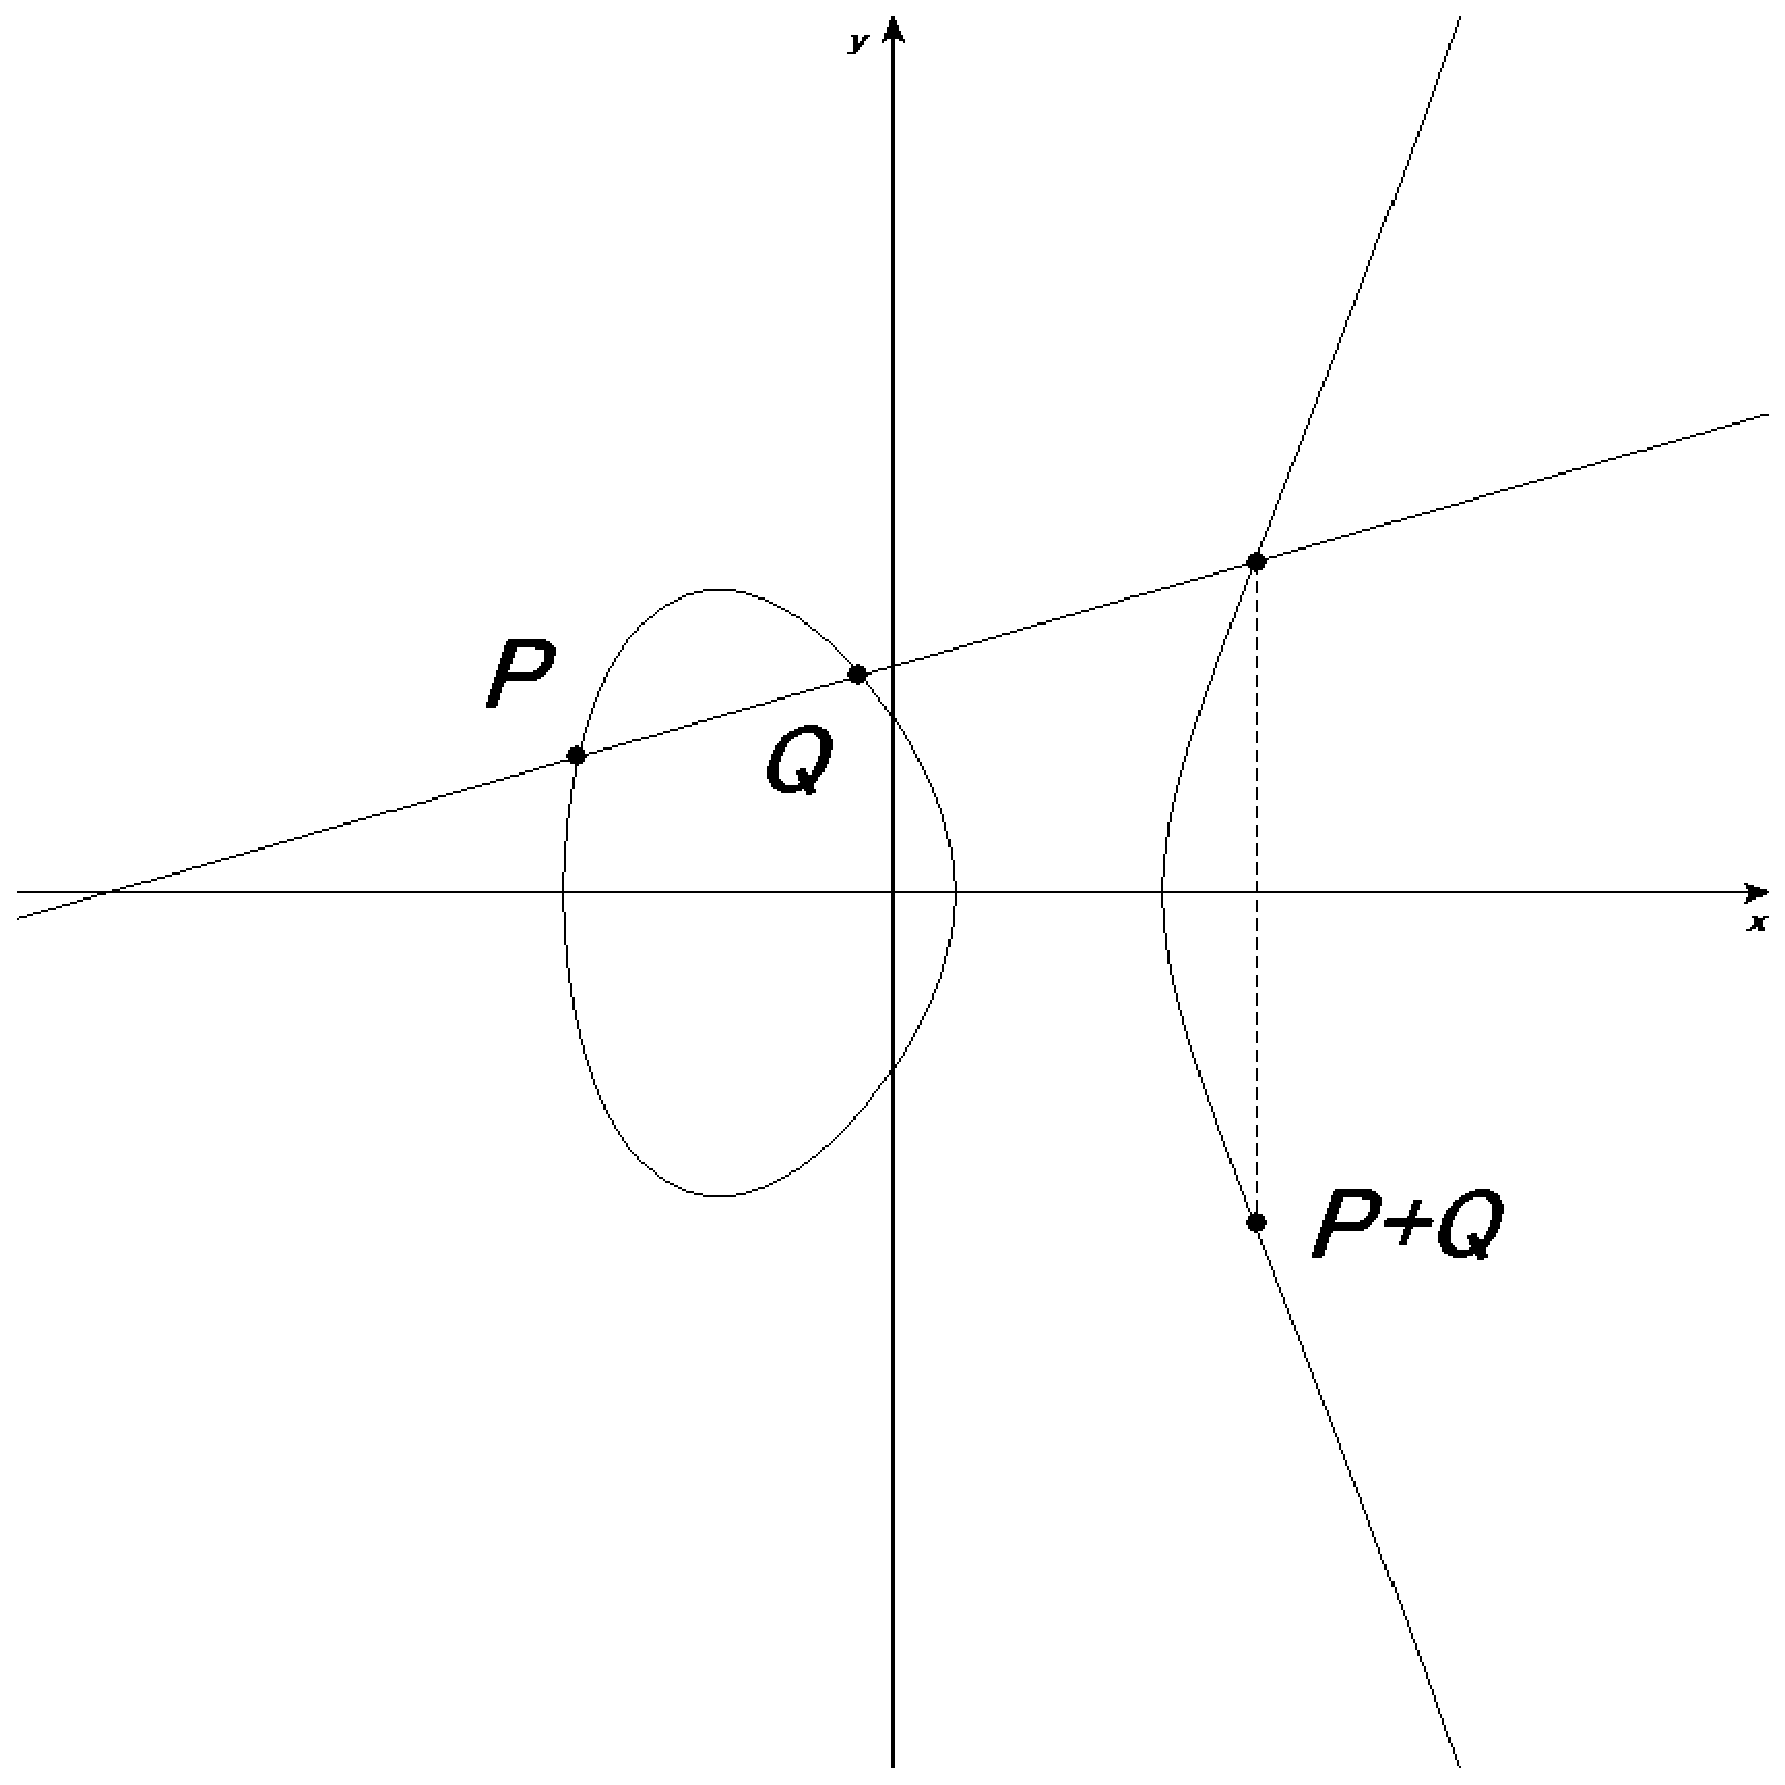
\includegraphics[width=80mm]{elliptic01.eps}
    \end{center}
    \caption{$P+Q$}
    \label{fig:elliptic01.eps}
  \end{minipage}
  \begin{minipage}{0.5\hsize}
    \begin{center}
      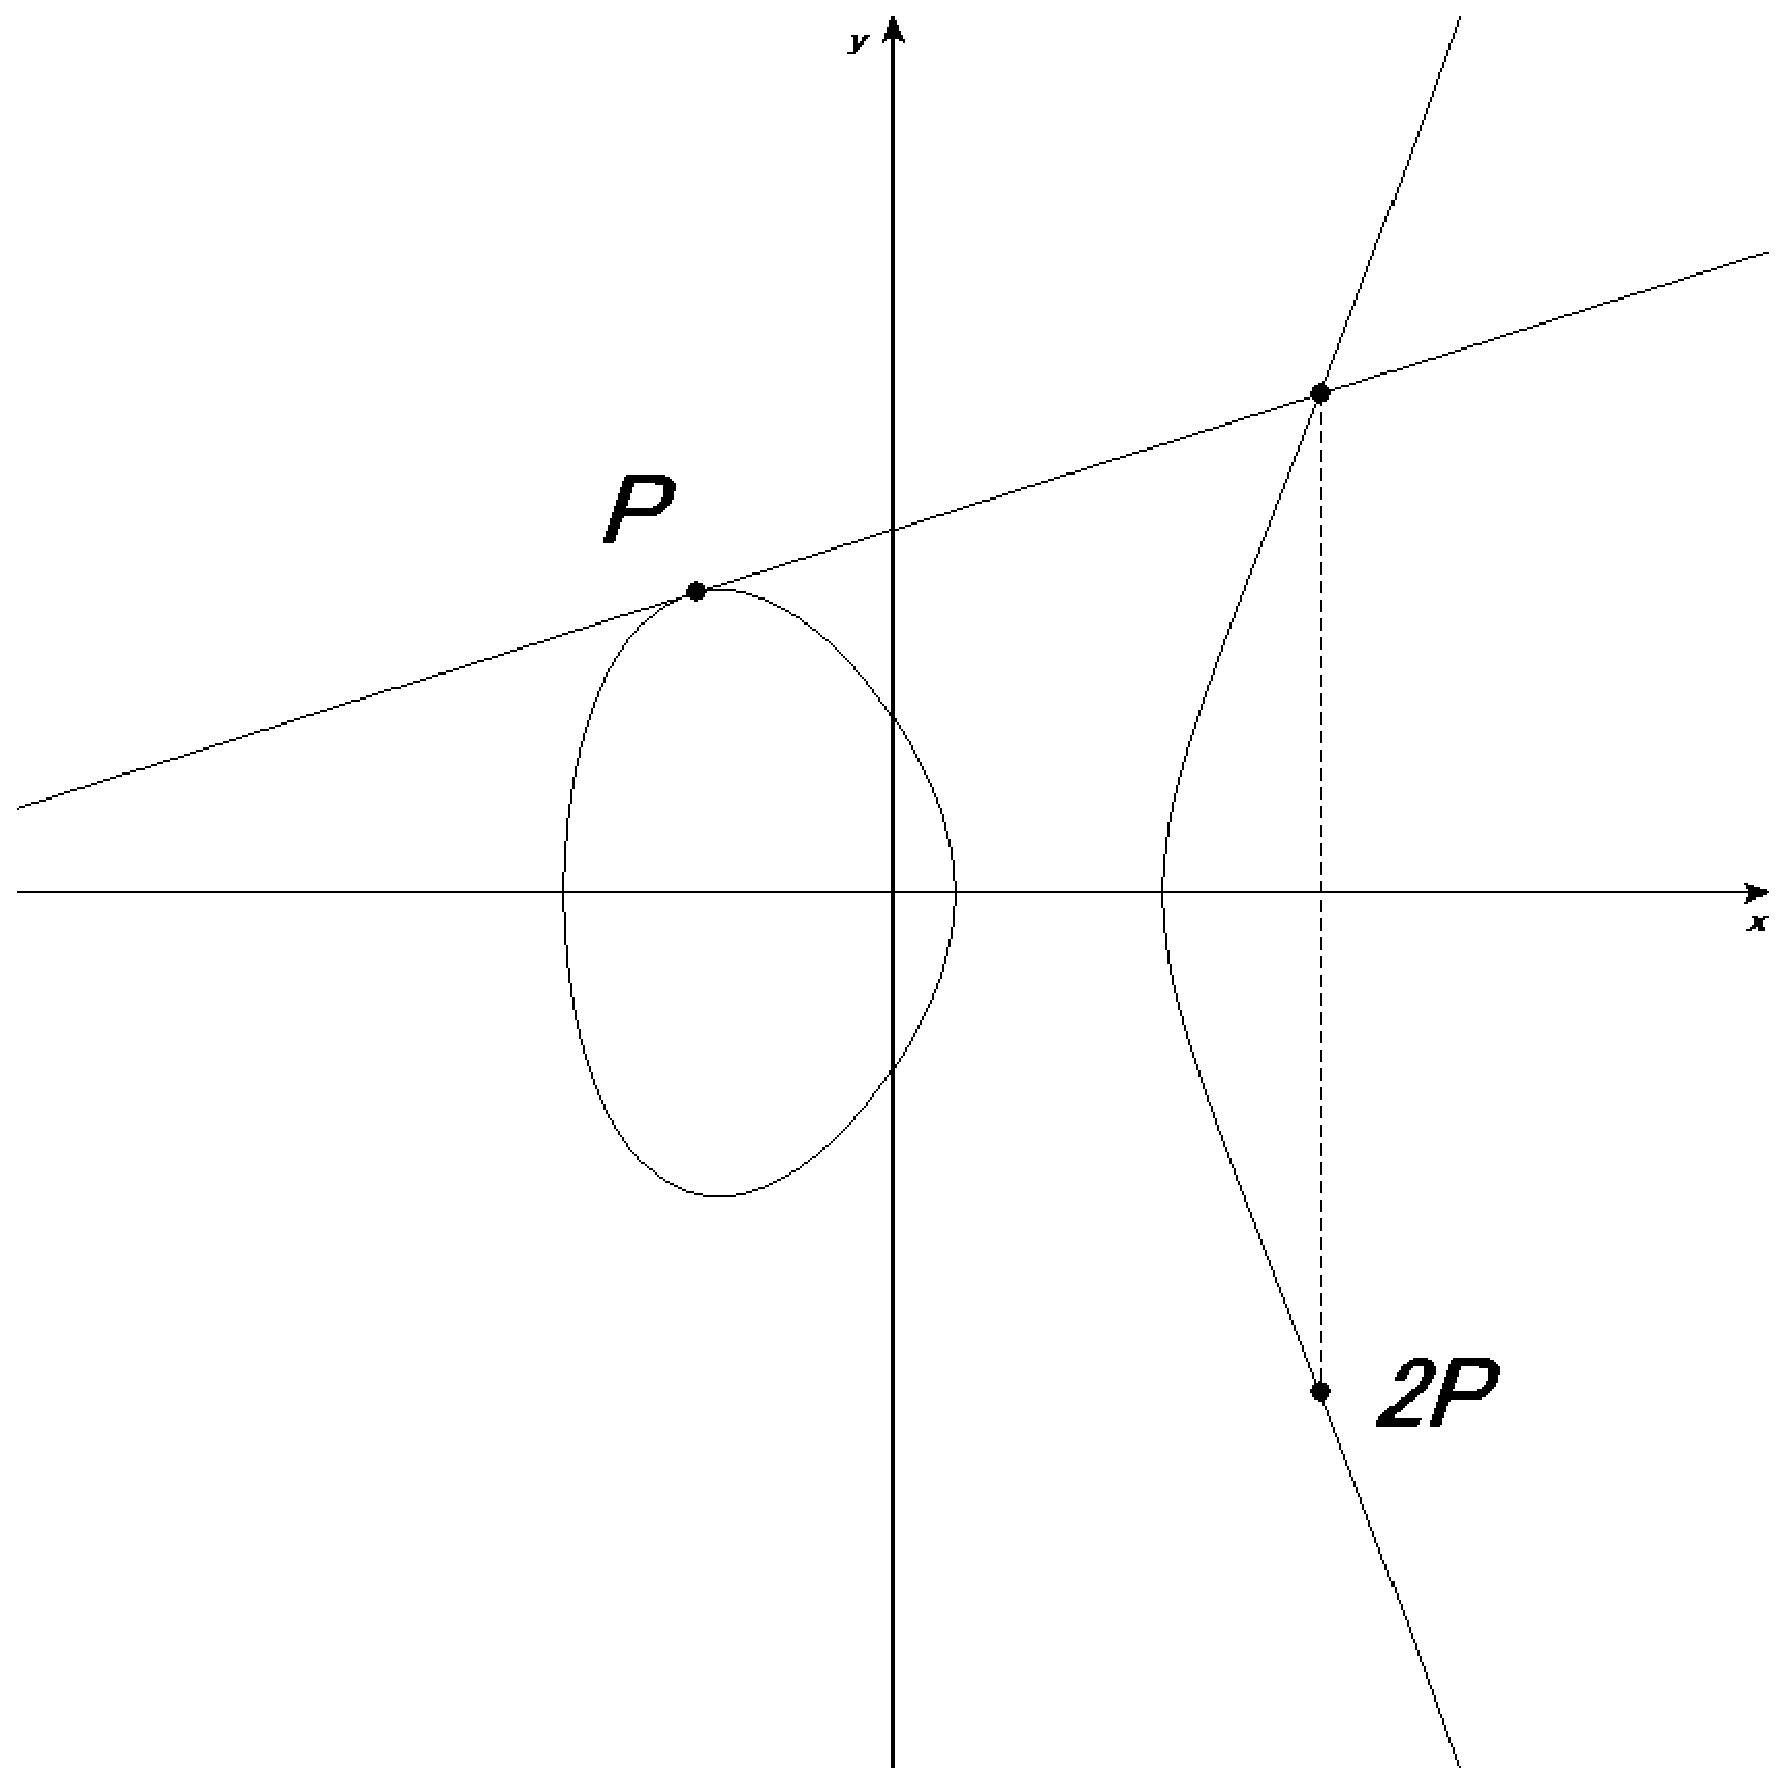
\includegraphics[width=80mm]{elliptic02.eps}
    \end{center}
    \caption{$2P$}
    \label{fig:elliptic02.eps}
  \end{minipage}
\end{figure}
\begin{figure}[htbp]
  \begin{minipage}{0.5\hsize}
    \begin{center}
      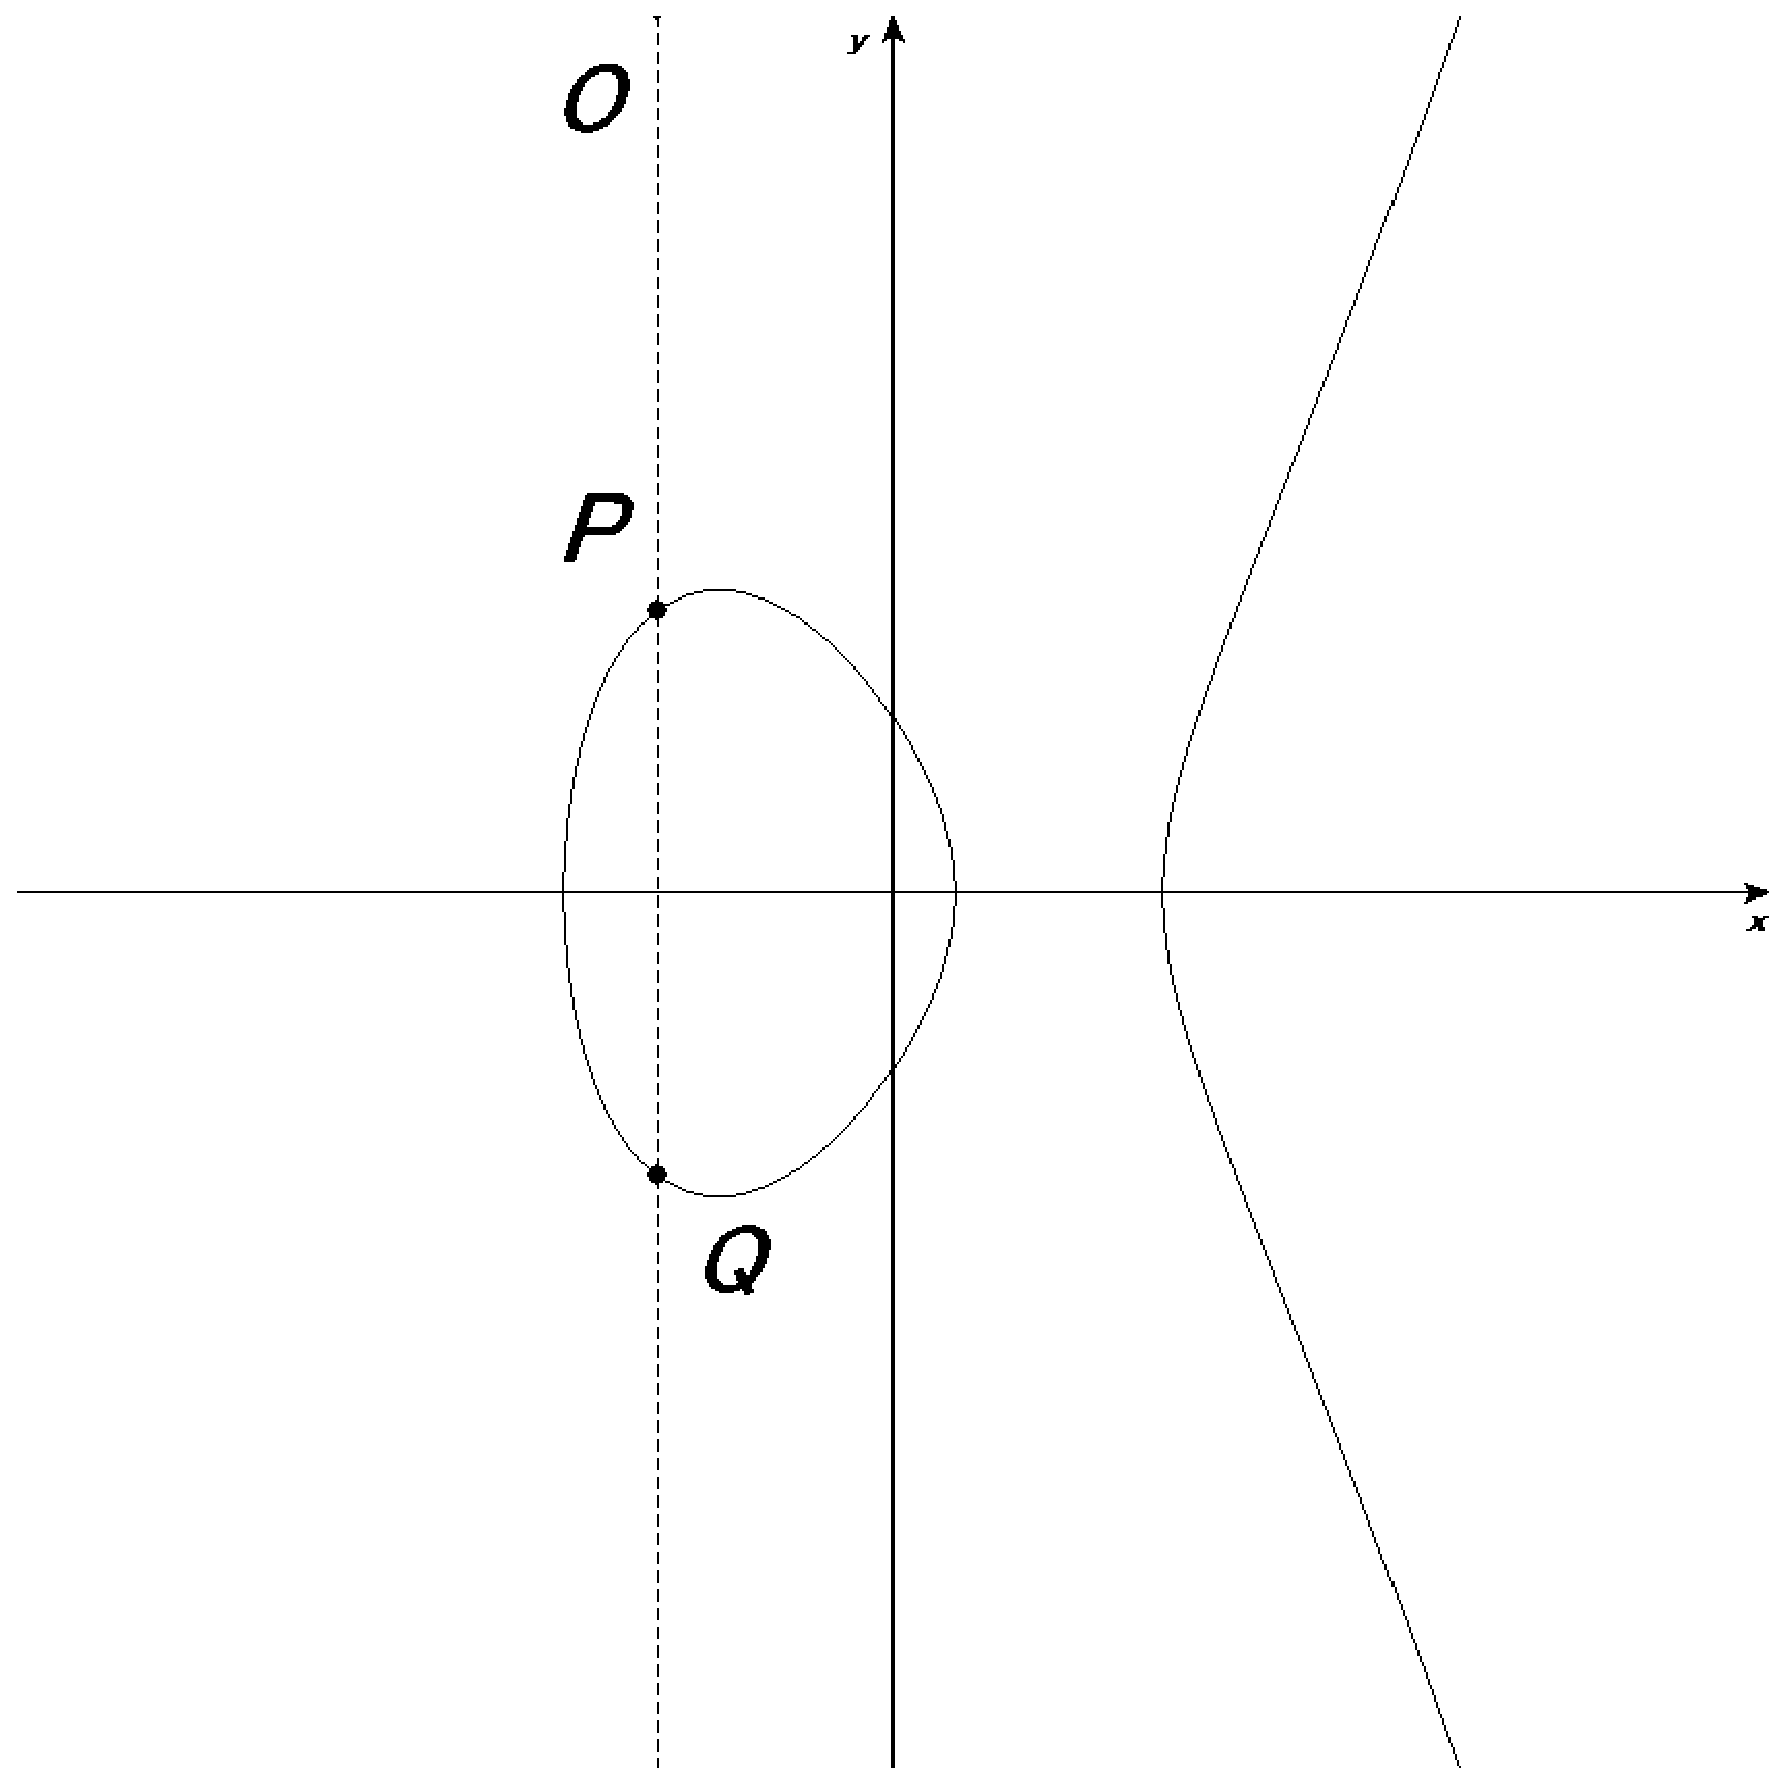
\includegraphics[width=80mm]{elliptic03.eps}
    \end{center}
    \caption{$P+Q=\mathcal{O}$}    \label{fig:elliptic03.eps}
  \end{minipage}
  \begin{minipage}{0.5\hsize}
    \begin{center}
      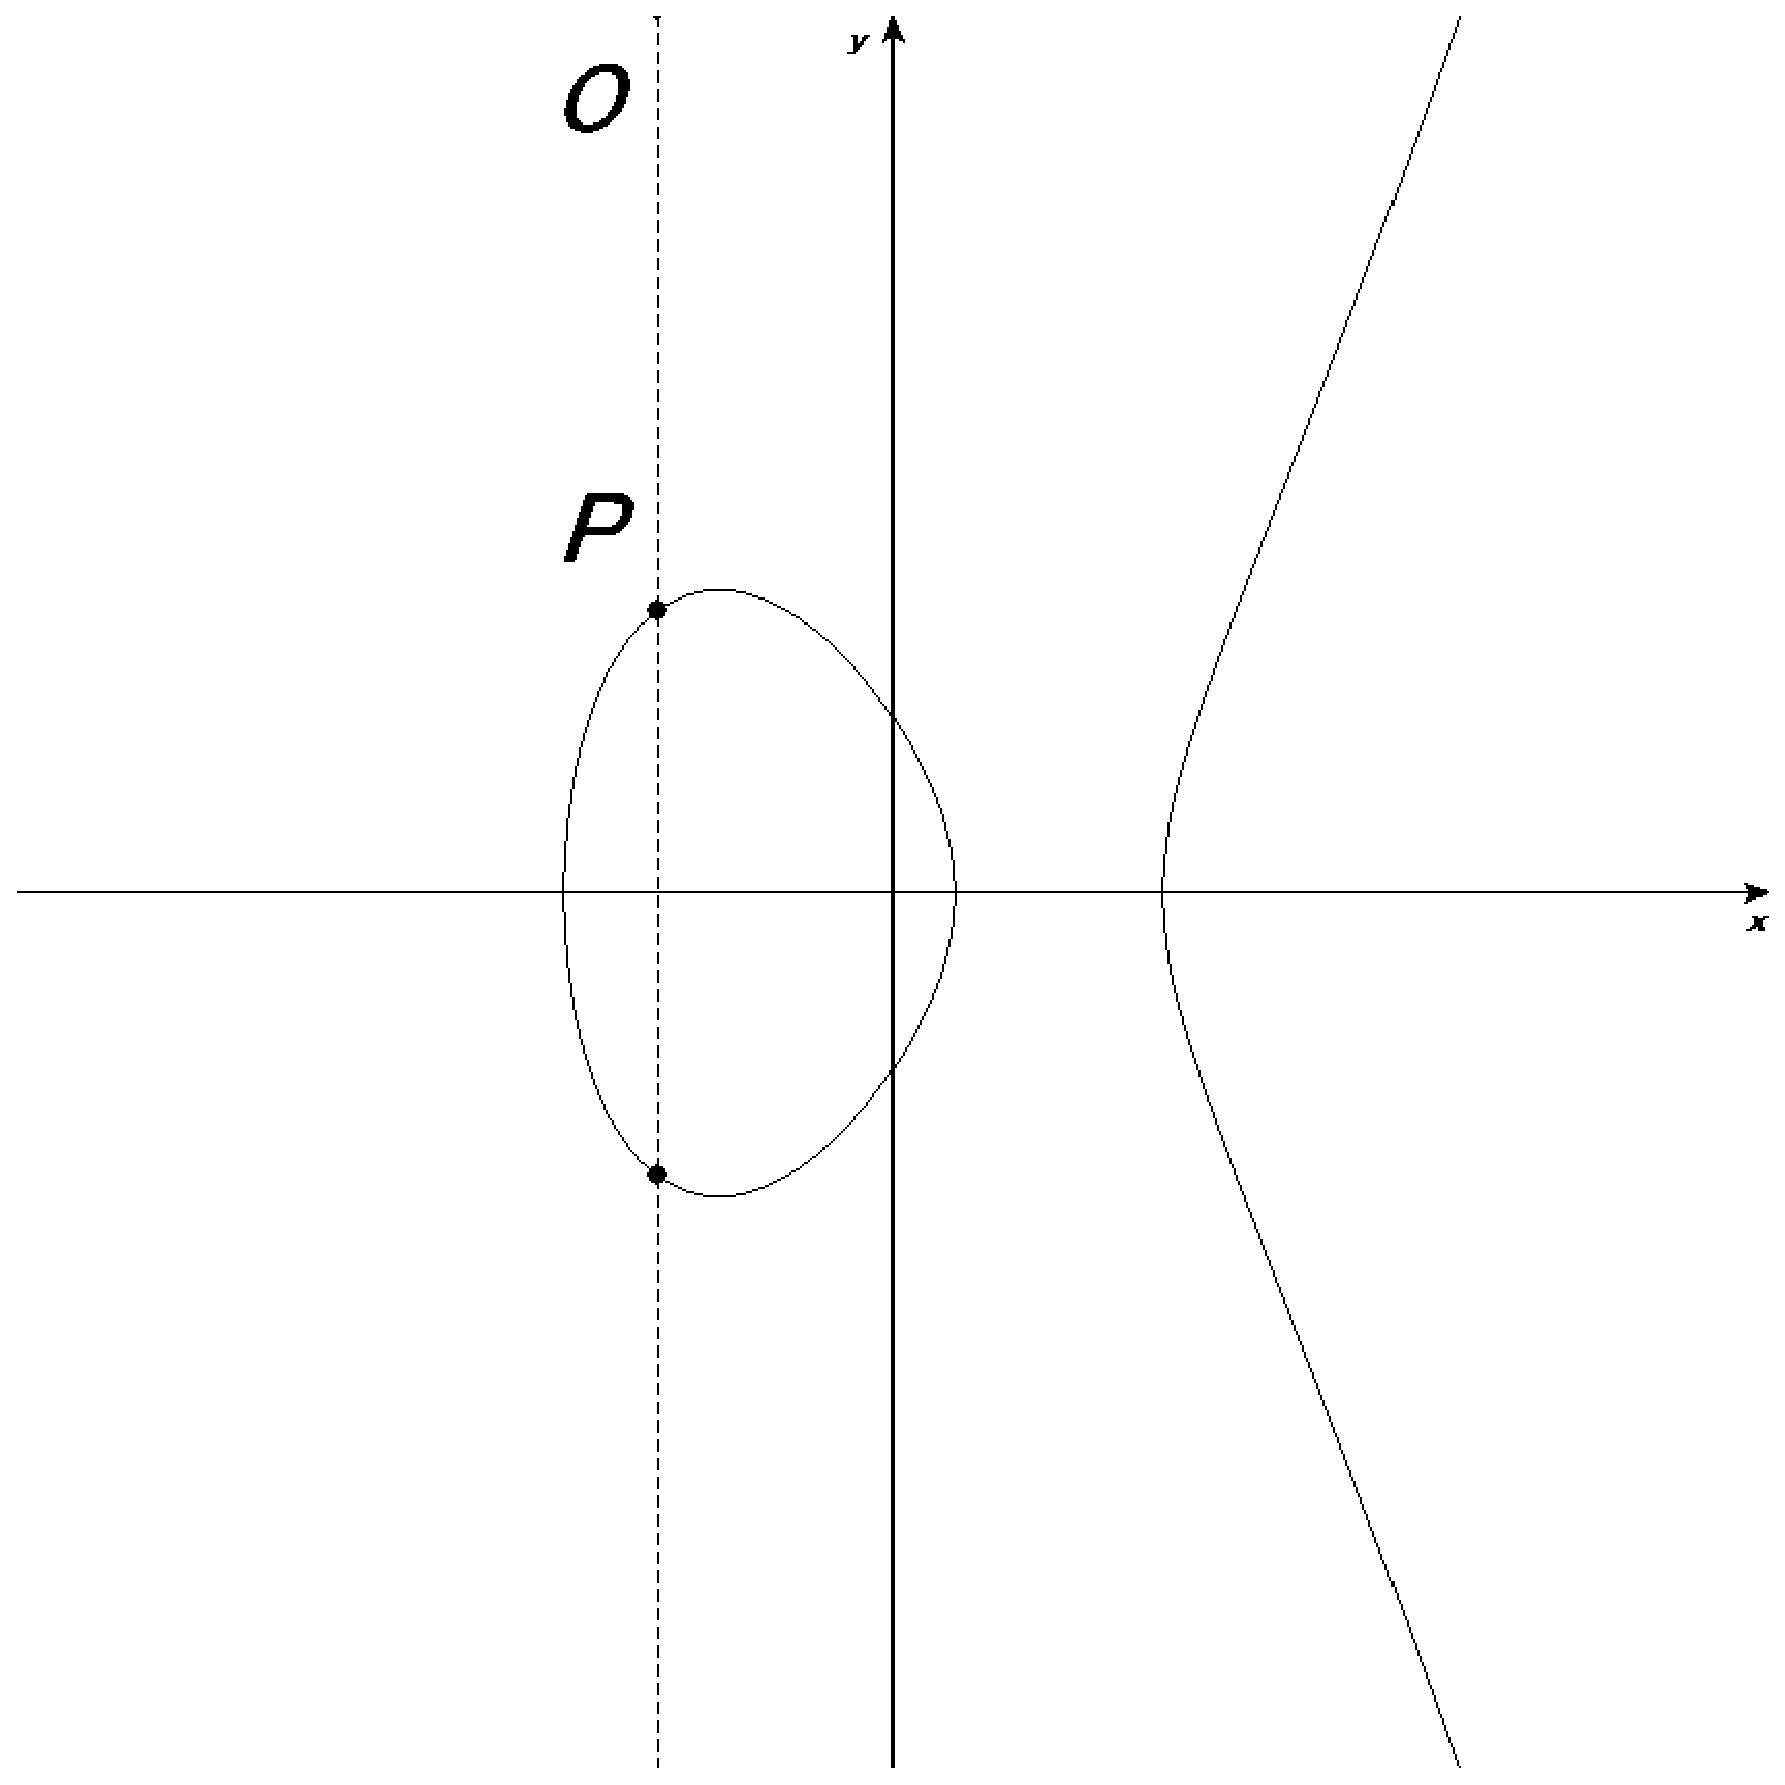
\includegraphics[width=80mm]{elliptic04.eps}
    \end{center}
    \caption{$P+\mathcal{O}=P$}
    \label{fig:elliptic04.eps}
  \end{minipage}
\end{figure}
\par
ここで,$P+Q$を効率的に計算できるよう公式を与える.
楕円曲線を$y^2 = x^3 + ax ^2 + bx +c$とし,各点を
\[
P _1 = (x _1, y _1), \quad P _2 = (x _2, y _2), \quad P*Q = (x _3, y _3), \quad P+Q = (x _3, - y _3)
\]
とする.
このとき,$P _1$と$P _2$を結ぶ直線の方程式は
\[
y = \lambda x + \nu, \quad \lambda = \frac{y _2 - y _1}{x _2 - x _1}, \quad \nu = y _1 - \lambda x _1 
\]
となり,これを楕円曲線の方程式に代入して
\[
x _3 = \lambda ^2 - a - x _1 - x _2, \quad y _3 = \lambda x _3 + \nu
\]
となる.
また,点$P$と点$P$の加算は,2倍算と定義され,$\lambda = \frac{f^{'}(x)}{2y}$を用いて2倍点の$x$座標は
\[
2倍点のx座標 = \frac{x^4 - 2bx^2 - 8cx + b^2 - 4ac}{4x^3 + 4ax^2 + 4bx + 4c}
\]
と表される.\\
\par
\section{楕円離散対数問題}
\subsection{離散対数問題(DLP)}
\par
$p$を素数とし,$g$を$\mathbb{Z}_p^*$の生成元とする.
このとき任意の$y\in \mathbb{Z}_p^*$に対し,
\[
y\equiv g^x\pmod{p}
\]
となる$x$が必ず存在する.
このような$x$を$y$の離散対数という.$y$と$g$が与えられたとき,$y\equiv g^x\pmod{p}$を満たす$x$,
すなわち$x\equiv \log _gy\pmod{p}$を求める問題を離散対数問題という.これは,$y\equiv g^x\pmod{p}$を計算するのは容易だが,$x\equiv \log _gy\pmod{p}$を
求めることは非常に困難であることに基づいている.
\par
\subsection{楕円離散対数問題(ECDLP)}
\par
任意の点$P\in E(\mathbb{F}_q)$に対して,
$\langle P\rangle =\{\mathcal{O},P,2P,3P,\ldots \}$は有限巡回群となる.
この巡回群の位数を$n$
とすると任意の$Q\in \langle P\rangle$に対して,
\[
xP=Q\ \ \ x\in (\mathbb{Z}_n)
\]
となる$x$がただ一つ存在する.
$P$と$Q$が与えられたとき,$x$を求める問題を楕円離散対数問題という.
これは$x$と$P$から$xP=Q$となる$Q$を求めるのは簡単だが,
$P$と$Q$から$x$を求めるのは非常に困難であることに基づいている.\\
\par
